
\section{To‘g‘ri chiziqli tekis harakatni grafik ravishda tasvirlash}

\begin{enumerate}

\item Rasmda bola bosib o‘tgan yo‘lning vaqtga bog‘lanish grafigi keltirilgan. 
Bolaning $t_1=1$ s va $t_2=5$ s vaqt oralig‘ida bosib o‘tgan yo‘lini aniqlang.


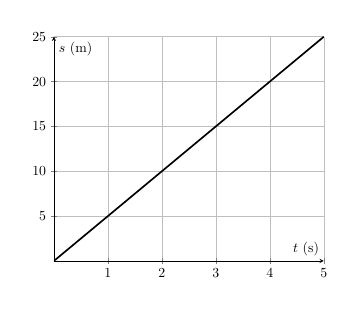
\begin{tikzpicture}[scale=0.5]
\begin{axis}[
axis lines=middle,
xlabel={$t$ (s)},
ylabel={$s$ (m)},
xmin=0,xmax=5,
ymin=0,ymax=25,
grid=both
]

\addplot[very thick] coordinates {
(0,0)
(1,5)
(2,10)
(3,15)
(4,20)
(5,25)
};

\end{axis}
\end{tikzpicture}


\begin{enumerate}[label=\Alph*)]
\item 10 m
\item 20 m
\item 5 m
\item 15 m
\end{enumerate}

\item Rasmda velosipedchi o‘tgan yo‘lning vaqtga bog‘lanish grafigi keltirilgan. 
Uning $t=4.28$ s vaqt momentidagi tezligi qanday (m/s)?


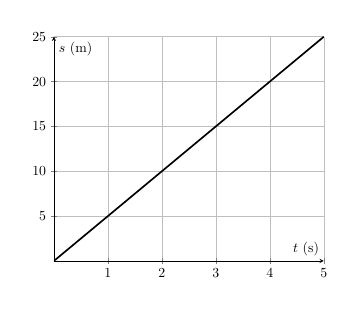
\begin{tikzpicture}[scale=0.5]
\begin{axis}[
axis lines=middle,
xlabel={$t$ (s)},
ylabel={$s$ (m)},
xmin=0,xmax=5,
ymin=0,ymax=25,
grid=both
]

\addplot[very thick] coordinates {
(0,0)
(1,5)
(2,10)
(3,15)
(4,20)
(5,25)
};

\end{axis}
\end{tikzpicture}


\begin{enumerate}[label=\Alph*)]
\item 5
\item 12
\item 10
\item 6

\end{enumerate}

\item Rasmda uchta moddiy nuqta bosib o‘tgan yo‘lning vaqtga bog‘lanish grafigi berilgan. 
Qaysi moddiy nuqtaning tezligi eng katta?


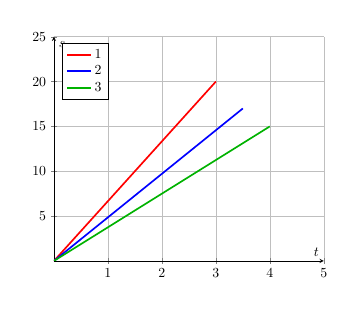
\begin{tikzpicture}[scale=0.5]
\begin{axis}[
axis lines=middle,
xlabel={$t$},
ylabel={$s$},
xmin=0,xmax=5,
ymin=0,ymax=25,
legend pos=north west,
grid=both
]

\addplot[very thick, red] coordinates {(0,0)(3,20)};
\addlegendentry{$1$}

\addplot[very thick, blue] coordinates {(0,0)(3.5,17)};
\addlegendentry{$2$}

\addplot[very thick, green!70!black] coordinates {(0,0)(4,15)};
\addlegendentry{$3$}

\end{axis}
\end{tikzpicture}


\begin{enumerate}[label=\Alph*)]
\item 1
\item 2
\item 3
\item hammasiniki bir xil

\end{enumerate}

\item Quyidagi grafikdan foydalanib jismning harakat tezligini aniqlang (m/s).


\begin{tikzpicture}[scale=0.6]
\draw[->] (0,0) -- (4,0) node[right] {$t$};
\draw[->] (0,0) -- (0,3) node[above] {$s$};

\draw (0,0) -- (3,2);

\draw (0.8,0) arc (0:30:0.8);
\node at (1.5,0.4) {$30^\circ$};

\node at (-0.1,-0.1) {$0$};
\end{tikzpicture}


\begin{enumerate}[label=\Alph*)]
\item $\sqrt{3}$
\item $\frac{\sqrt{3}}{3}$
\item 3
\item $\frac{1}{2}$

\end{enumerate}

\item Qaysi grafik jism o‘tgan yo‘lning vaqtga bog‘lanishini ifodalay olmaydi?

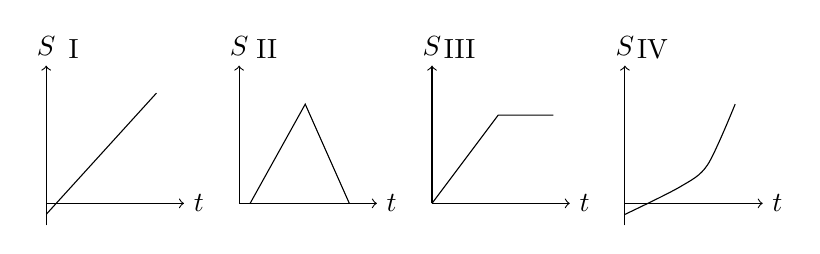
\begin{tikzpicture}[scale=0.7]

% I
\begin{scope}
\node at (0.5,2.8) {I};
\draw[->] (0,0) -- (2.5,0) node[right] {$t$};
\draw[->] (0,-0.4) -- (0,2.5) node[above] {$S$};
\draw (0,-0.2) -- (2,2);
\end{scope}

% II
\begin{scope}[xshift=3.5cm]
\node at (0.5,2.8) {II};
\draw[->] (0,0) -- (2.5,0) node[right] {$t$};
\draw[->] (0,0) -- (0,2.5) node[above] {$S$};
\draw (0.2,0) -- (1.2,1.8) -- (2,0);
\end{scope}

% III
\begin{scope}[xshift=7cm]
\node at (0.5,2.8) {III};
\draw[->] (0,0) -- (2.5,0) node[right] {$t$};
\draw[->] (0,0) -- (0,2.5) node[above] {$S$};
\draw (0,0) -- (1.2,1.6) -- (2.2,1.6);
\end{scope}

% IV
\begin{scope}[xshift=10.5cm]
\node at (0.5,2.8) {IV};
\draw[->] (0,0) -- (2.5,0) node[right] {$t$};
\draw[->] (0,-0.4) -- (0,2.5) node[above] {$S$};
\draw plot[smooth] coordinates {(0,-0.2)(1,0.3)(1.5,0.7)(2,1.8)};
\end{scope}

\end{tikzpicture}

\begin{enumerate}[label=\Alph*)]
\item II, III
\item I, II, IV
\item III
\item I, IV

\end{enumerate}

\item Chizmada uchta moddiy nuqtaning harakat grafiklari berilgan. 
Ularning tezliklari haqida nima deyish mumkin?


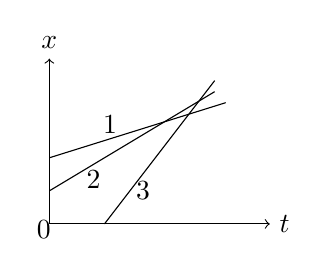
\begin{tikzpicture}[scale=0.7]

\draw[->] (0,0) -- (4,0) node[right] {$t$};
\draw[->] (0,0) -- (0,3) node[above] {$x$};

\draw (0,1.2) -- (3.2,2.2);
\draw (0,0.6) -- (3,2.4);
\draw (1,0) -- (3,2.6);

\node at (1.1,1.8) {1};
\node at (0.8,0.8) {2};
\node at (1.7,0.6) {3};

\node at (-0.1,-0.1) {$0$};

\end{tikzpicture}


\begin{enumerate}[label=\Alph*)]
\item $v_1<v_2<v_3$
\item $v_1>v_2>v_3$
\item $v_1=v_2=v_3$
\item $v_1=v_2>v_3$
\end{enumerate}

\item Grafikdan foydalanib OX o‘q bo‘ylab harakat qilayotgan moddiy nuqtaning 
5 s da bosib o‘tgan yo‘lini aniqlang (m).


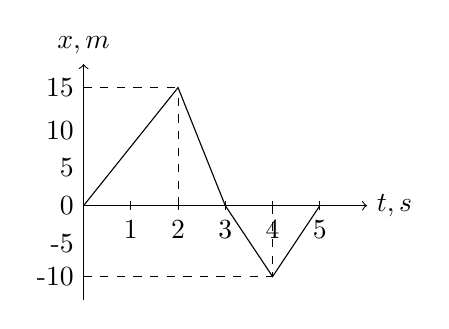
\begin{tikzpicture}[scale=0.6]

\draw[->] (0,-2) -- (0,3) node[above] {$x,m$};
\draw[->] (0,0) -- (6,0) node[right] {$t,s$};

\draw (0,0) -- (2,2.5) -- (3,0) -- (4,-1.5) -- (5,0);

\draw[dashed] (2,0) -- (2,2.5);
\draw[dashed] (0,2.5) -- (2,2.5);

\draw[dashed] (4,0) -- (4,-1.5);
\draw[dashed] (0,-1.5) -- (4,-1.5);

\node[left] at (0,2.5) {15};
\node[left] at (0,1.6) {10};
\node[left] at (0,0.8) {5};
\node[left] at (0,0) {0};
\node[left] at (0,-0.8) {-5};
\node[left] at (0,-1.5) {-10};

\foreach \x in {1,2,3,4,5}
\draw (\x,0.1) -- (\x,-0.1) node[below] {\x};

\end{tikzpicture}


\begin{enumerate}[label=\Alph*)]
\item 50
\item 32.5
\item 0
\item 10
\end{enumerate}

\item Rasmda jism koordinatasining vaqtga bog‘liqlik grafigi berilgan. 
Jismning harakat tenglamasini yozing.


\begin{tikzpicture}[scale=0.6]

\draw[->] (0,0) -- (6,0) node[right] {$t,s$};
\draw[->] (0,-1) -- (0,3.5) node[above] {$x,m$};

\draw (0,3) -- (4,-1);

\node[left] at (0,3) {6};
\node[left] at (0,1.5) {3};

\foreach \x in {1,2,3,4,5}
\draw (\x,0.1) -- (\x,-0.1) node[below] {\x};

\end{tikzpicture}


\begin{enumerate}[label=\Alph*)]
\item $x=-2+4t$
\item $x=6+3t$
\item $x=-6+3t$
\item $x=6-2t$

\end{enumerate}

\item Rasmda jismning harakat grafigi keltirilgan. 
$t=3$ s paytdagi jismning koordinatasini aniqlang (m).


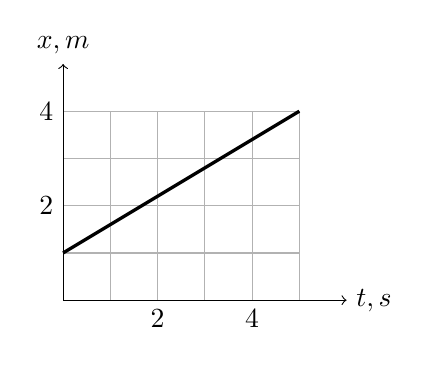
\begin{tikzpicture}[scale=0.6]

\draw[step=1cm,gray!60] (0,0) grid (5,4);

\draw[->] (0,0) -- (6,0) node[right] {$t,s$};
\draw[->] (0,0) -- (0,5) node[above] {$x,m$};

\draw[very thick] (0,1) -- (5,4);

\node[left] at (0,4) {4};
\node[left] at (0,2) {2};

\node[below] at (2,0) {2};
\node[below] at (4,0) {4};

\end{tikzpicture}


\begin{enumerate}[label=\Alph*)]
\item 1.8
\item 1.6
\item 2.8
\item 1.2
\end{enumerate}

\item Rasmda jism koordinatasining vaqtga bog‘lanish grafigi tasvirlangan. 
Jismning $(1-4)$ s vaqt oralig‘idagi ko‘chishini va yo‘lini aniqlang (m).


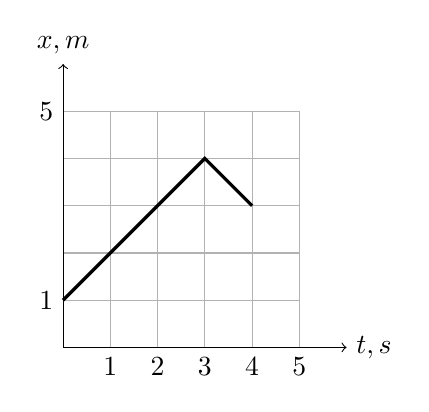
\begin{tikzpicture}[scale=0.6]

\draw[step=1cm,gray!60] (0,0) grid (5,5);

\draw[->] (0,0) -- (6,0) node[right] {$t,s$};
\draw[->] (0,0) -- (0,6) node[above] {$x,m$};

\draw[very thick] (0,1) -- (3,4) -- (4,3);

\node[left] at (0,5) {5};

\foreach \x in {1,2,3,4,5}
\node[below] at (\x,0) {\x};

\node[left] at (0,1) {1};

\end{tikzpicture}


\begin{enumerate}[label=\Alph*)]
\item 1; 4
\item 2; 4
\item 1; 3
\item 2; 3
\end{enumerate}

\item Rasmda jismning harakat grafigi ko‘rsatilgan. Grafikning qaysi qismida jismning tezligi eng katta bo‘lgan?


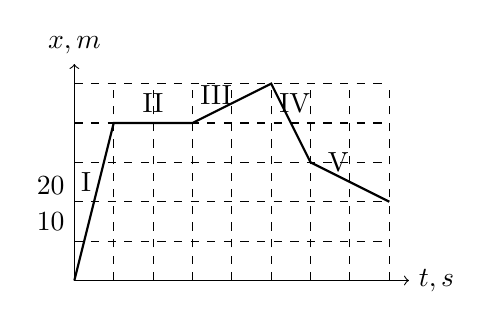
\begin{tikzpicture}[scale=0.5]

\draw[->] (0,0) -- (8.5,0) node[right] {$t,s$};
\draw[->] (0,0) -- (0,5.5) node[above] {$x,m$};

\draw[step=1cm,dashed] (0,0) grid (8,5);

\node[left] at (0,1.5) {10};
\node[left] at (0,2.4) {20};

\draw[thick]
(0,0) --
(1,4) --
(3,4) --
(5,5) --
(6,3) --
(8,2);

\node at (0.3,2.5) {I};
\node at (2,4.5) {II};
\node at (3.6,4.7) {III};
\node at (5.6,4.5) {IV};
\node at (6.7,3) {V};

\end{tikzpicture}


\begin{enumerate}[label=\Alph*)]
\item III
\item II
\item I
\item IV
\end{enumerate}

\item Chizmada keltirilgan tezlik grafigidan foydalanib X o‘qi bo‘ylab 
harakatlanayotgan jismning harakat tenglamasini tuzing. 
Boshlang‘ich koordinata $-10$ m.

\begin{center}
\begin{tikzpicture}[scale=0.6]

% o'qlar
\draw[->] (0,0) -- (5,0) node[right] {$t$};
\draw[->] (0,0) -- (0,3) node[above] {$v,\;m/s$};

% belgilar
\node[left] at (0,2) {4};
\node[below left] at (0,0) {0};

% tezlik chizig'i
\draw[thick] (0,2) -- (4,2);

\end{tikzpicture}
\end{center}


\begin{enumerate}[label=\Alph*)]
\item $x=-10+4t$
\item $x=-10+2t^2$
\item $x=-10t+4t^2$
\item $x=-10+2t$
\end{enumerate}

\end{enumerate}




\begin{table}[h!]
\centering
\begin{tabular}{|c|c|c|c|c|c|c|c|c|c|}
\hline
1b & 2a & 3a & 4b & 5c & 6c & 7a & 8d & 9d & 10b \\ \hline
11c & 12a &  &  &  &  &  &  &  &  \\ \hline
\end{tabular}
\end{table}




